\subsection{Hinführung zum Thema}
\label{sub:hinführung_zum_thema}
    Datenvisualisierung ist ein Thema, das nicht nur in jüngster Zeit sehr viel Zuwendung fand, sondern auch für die Analyse verschiedenster Sachverhalte immer wichtiger wird. So lassen sich komplexe Zusammenhänge eines Systems oftmals erst dann richtig begreifen, wenn wir alle möglichen Zustände davon erfassen können. In "`Up and Down the Ladder of Abstraction"', beschreibt Bret Victor, wie sich Systeme in ihrer Ganzheit besser begreifen und gestalten lassen.

    \begin{quote}
        \emph{"`When designing [a system], the challenge lies not in constructing the system, but in understanding it. In the absence of theory, we must develop an intuition to guide our decisions. The design process is thus one of exploration and discovery."'} \parencite{victor}
    \end{quote}

    Auch eine Ansammlung an Daten ist erst einmal sehr abstrakt. In einer Datenbank in Relation gebracht, bleiben die meisten Erkenntnisse und Stories hinter diesen Daten verborgen. Ein tieferes Verständnis erhalten wir erst dann, wenn wir sie auswerten. Eine mögliche Form einer solchen Auswertung stellt die Datenvisualisierung dar. Die Art der Datenvisualisierung hat sich dabei in den letzten Jahren stark gewandelt. Während Daten anfangs vor allem in Form von Häufigkeitsanalysen ausgewertet und als Bar- oder Linechart visualisiert wurden, finden wir heute vermehrt interaktive Karten, mit denen raumbezogene Zusammenhänge veranschaulicht werden können. Dieser Trend von dynamischen Live-Visualisierungen fand in verschiedensten Bereichen Einzug. Zum Beispiel der erst kürzlich erschienene Flight-Planner des Dubai Airports\footnote{\url{http://www.dubaiairports.ae/flight-planner}}, die Marine-Traffic-Map\footnote{\url{https://www.marinetraffic.com/}} in der Schifffahrt oder auch für die Live-Simulation von Wetterdaten\footnote{\url{https://www.windy.com/}}.\\

    Auch hier in Deutschland gibt es verschiedene Produkte, die veröffentlicht wurden. Beispielsweise der Zugradar\footnote{\url{http://bahn.de/zugradar}} (2014) und der Busradar\footnote{\url{https://play.google.com/store/apps/details?id=de.hafas.android.dbbusradar}} der Deutschen Bahn oder eine Karte für das S-Bahn Netz in München\footnote{\url{http://s-bahn-muenchen.hafas.de/}} (2009).

    Eine gesamte Erfassung des Öffentlichen Verkehrs ging ebenfalls 2014 mit Travic\footnote{\url{http://tracker.geops.de/}}\label{travic} online und bietet mit über 650 integrierten Fahrplänen eine enorme Abdeckung. Da die Live-Karten der Deutschen Bahn damals nur die Visualisierung der eigenen Bus- und Bahnlinien ermöglichte, war Travic bestrebt, diese Lücke zu schließen und den gesamten Öffentlichen Verkehr darzustellen. 
    Zusätzlich sei noch LiveMap24 \footnote{\url{https://www.livemap24.com/}} von Verdict erwähnt, deren Veröffentlichungsdatum allerdings nicht bekannt ist.\\

    Der Vorteil einer digitalen Karte besteht in seiner ständigen Aktualität. Ein statischer Fahrplan kann keine Informationen zu Störungen, Verspätungen oder Ausfall eines Zuges geben. Auf einer Live-Karte lassen sich solche Informationen visuell aufbereiten und dem Anwender über die Benutzeroberfläche vermitteln. Der Betrachter kann einsehen, wie viele Fahrzeuge gerade aktiv sind und kann zusätzlich zum statischen Fahrplan auch visuell erleben, wo sich sein Zug oder Bus befindet. 
    Da gleichzeitig Fahrplan als auch Karte vorhanden sind, ist auch eine geographische Orientierung möglich. Dem Satz \emph{"`Der Zug hat 5 Minuten Verspätung"'} wird ein visueller Kontext gegeben und ist dadurch nicht mehr nur eine Aussage, sondern wird visuell erfahrbar.
    Den Mehrwert einer Live-Karte sehen wohl aber nicht nur Pendler oder Reisende, sondern auch Verkehrsunternehmen, Städteplaner oder Verkehrsforscher.\\

    Diese Arbeit befasst sich umfassend mit der Entwicklung einer Live-Karte für den Öffentlichen Nahverkehr im Raum Stuttgart als Webanwendung. Der Fokus liegt dabei auf der Exploration verschiedener Visualisierungen und Funktionen, welche die Karte interaktiv gestalten und gleichzeitig die User-Experience erhöhen. Das Ergebnis dieses Vorhabens soll bereits vorab vorgestellt werden und ist deshalb als Screenshot in Abbildung \ref{fig:rtt-map} zu sehen.

    \begin{figure}[htbp]
        \begin{center}
            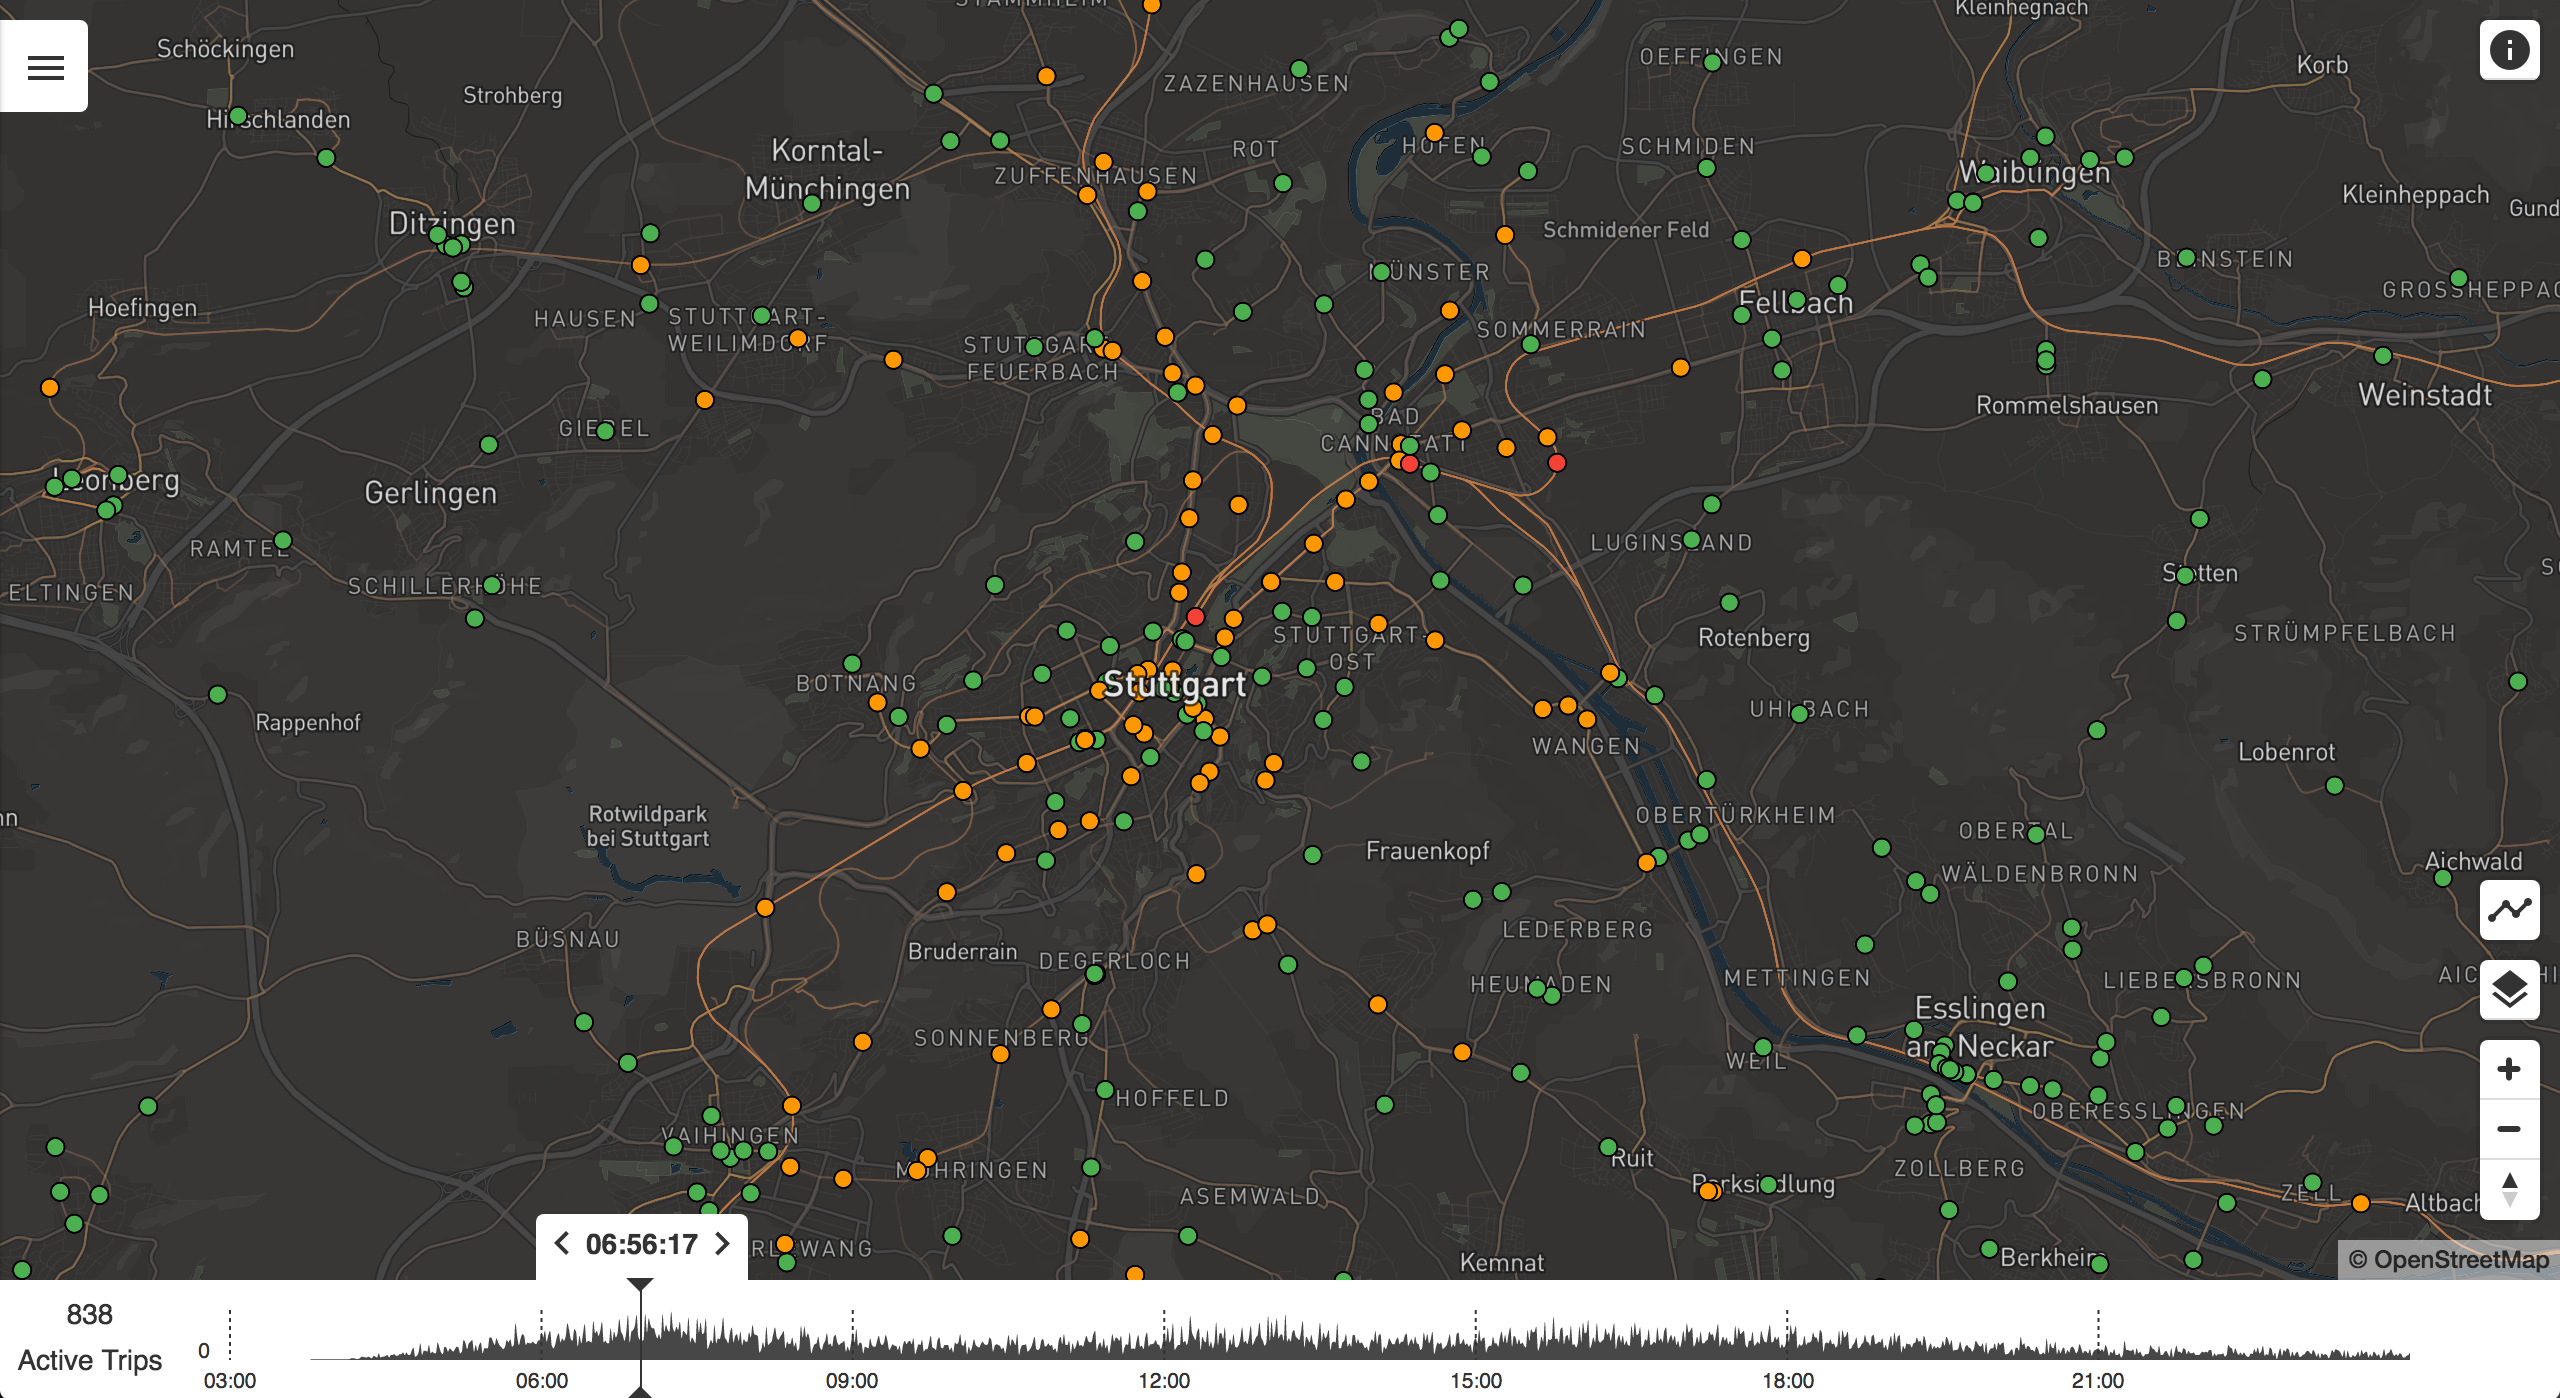
\includegraphics[width=0.99\textwidth]{rtt-map}
            \caption{Screenshot der fertigen Webanwendung}
            \label{fig:rtt-map}
        \end{center}
    \end{figure}
    
% subsection hinführung_zum_thema (end)